\documentclass[12pt]{article}
\usepackage{amsmath}
\usepackage{graphicx}
\usepackage{float}
\begin{document}
\title{Electrical Engineering 141, Homework 6}
\date{March 1st, 2019}
\author{Michael Wu\\UID: 404751542}
\maketitle

\section*{Problem 1}

The open loop transfer function is the following.
\[\frac{K}{(s+1)^3}\]
This crosses the real axis when \(1+j\omega\) has a phase of \(\pm \frac{\pi}{3}\) or \(0\). This occurs
at \(\omega=0,\pm\sqrt{3}\). The magnitude of the open loop transfer function at these points are
\(K\) and \(-\frac{K}{8}\), respectively. The open loop transfer function has no poles in the right half
plane, so we should have no encirclements around \(-1\) in order to have a stable system. Since we know
that the value of the transfer function goes to zero as \(\omega\) goes to \(\infty\), we know that we
will have an encirclement if \(-\frac{K}{8}<-1\). On the positive side we also know we will have an
encirclement if \(K<-1\). Thus we want the following inequality to hold in order to have a stable system.
\[-1<K<8\]

\section*{Problem 2}

\paragraph{a)}

The Nyquist diagram is shown below.
\begin{figure}[H]
    \begin{center}
        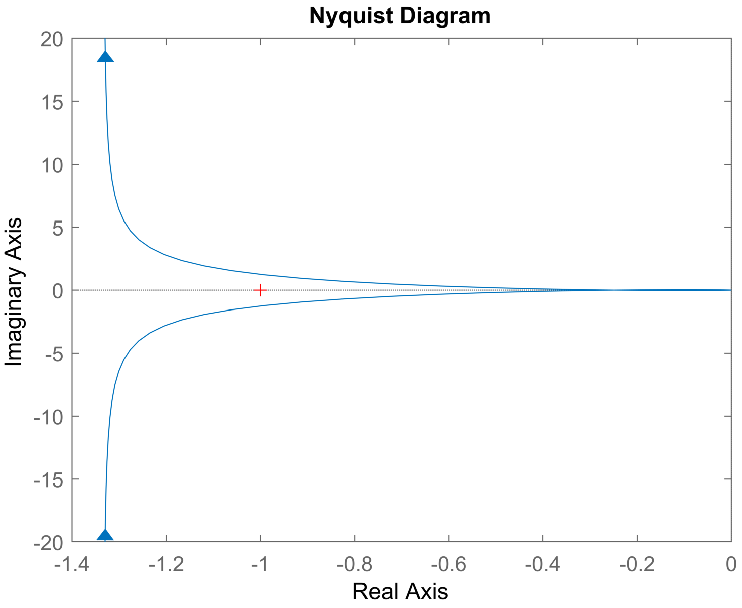
\includegraphics[width=3.5in]{problem2a.pdf}
    \end{center}
\end{figure}
The plot goes to infinity, and since we choose to not include the open loop pole at \(s=0\), we determine
that the loop connects on the right half plane. Thus the critical point is not contained within a loop, and
there are no unstable poles in the closed loop transfer function since the contour does not circle any open
loop poles.

\paragraph{b)}

The Nyquist plot crosses the real axis when \(j\omega(1+j\omega)(3+j\omega)\) is real. This can be rewritten
as the following expression.
\[-4\omega^2+j(3\omega-\omega^3)\]
This occurs when \(\omega=0,\pm \sqrt{3}\) and the corresponding magnitude of the transfer function is
\(K\infty\) and \(-\frac{K}{4}\). Thus we must have \(0<K<4\) in order to have a stable closed loop system.

\paragraph{c)}

If we have \(K>4\), then the critical point will have two clockwise loops around it. Then the Nyquist stability
criterion indicates that there will be two more closed loop poles than open loop poles in the right half plane.
Since we have zero open loop poles in the right half plane, this means there will be two closed loop poles in
the right half plane. If we have \(K<0\), then the critical point will have one clockwise loop around it. This corresponds
to one closed loop pole in the right half plane.

\paragraph{d)}

The root locus plot is shown below.
\begin{figure}[H]
    \begin{center}
        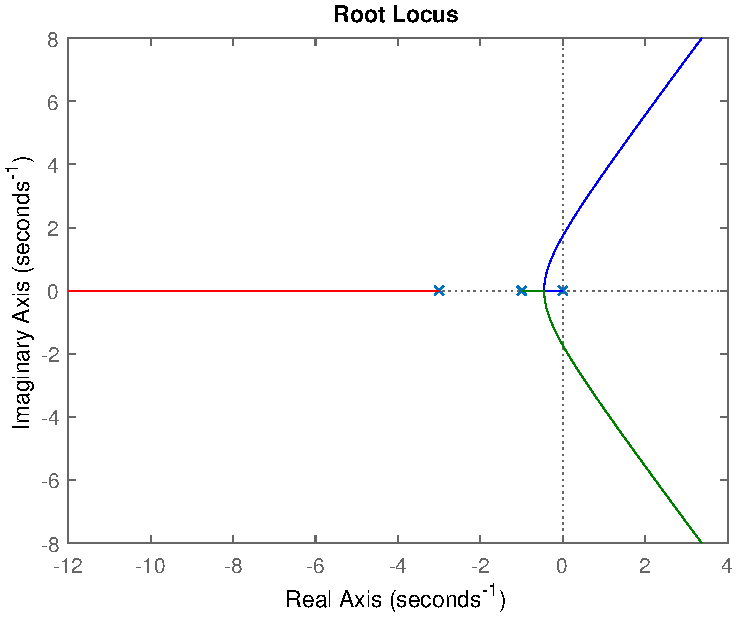
\includegraphics[width=3.5in]{problem2d-reg.pdf}
    \end{center}
\end{figure}
The complementary root locus plot is shown below.
\begin{figure}[H]
    \begin{center}
        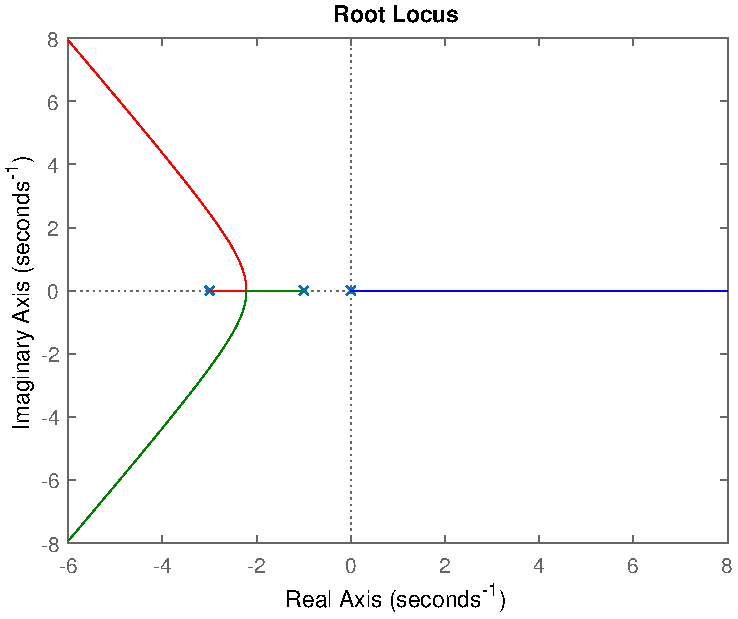
\includegraphics[width=3.5in]{problem2d-comp.pdf}
    \end{center}
\end{figure}
This confirms that there will be two unstable poles as \(K\) increases above \(4\). Clearly the complementary
root locus plot indicates that there will be one unstable real pole if \(K\) is negative.

\section*{Problem 3}

\paragraph{a)}

The shape of the Nyquist diagram is shown below.
\begin{figure}[H]
    \begin{center}
        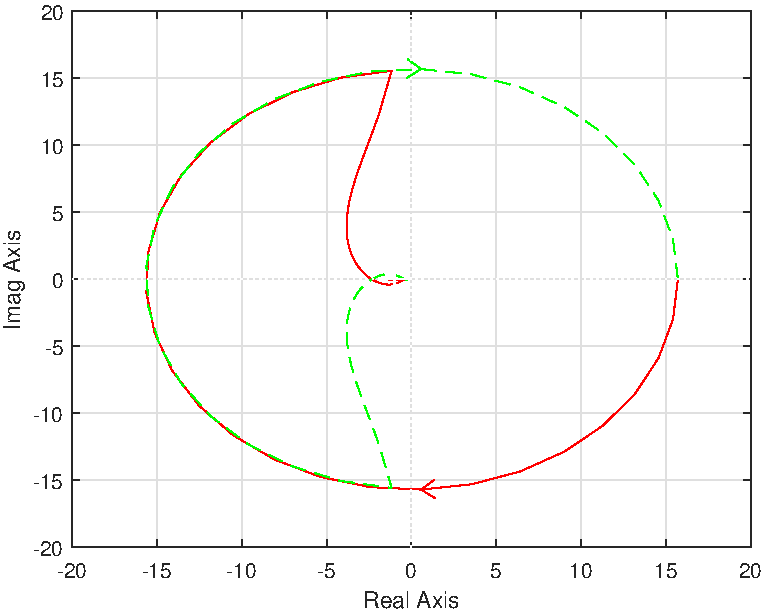
\includegraphics[width=3.5in]{problem3a.pdf}
    \end{center}
\end{figure}

\paragraph{b)}

The Nyquist diagram encircles the critical point zero times, since it encircles it once in the clockwise direction
and once in the counterclockwise direction. This means that our system is stable.

\paragraph{c)}

Using a calculator I found that the Nyquist plot crosses the real axis at \(-0.2843\) and \(-4.0705\). This corresponds to
the following upward and downward gain margin.
\[0.2457<K<3.517\]

\paragraph{d)}

The root locus is shown below.
\begin{figure}[H]
    \begin{center}
        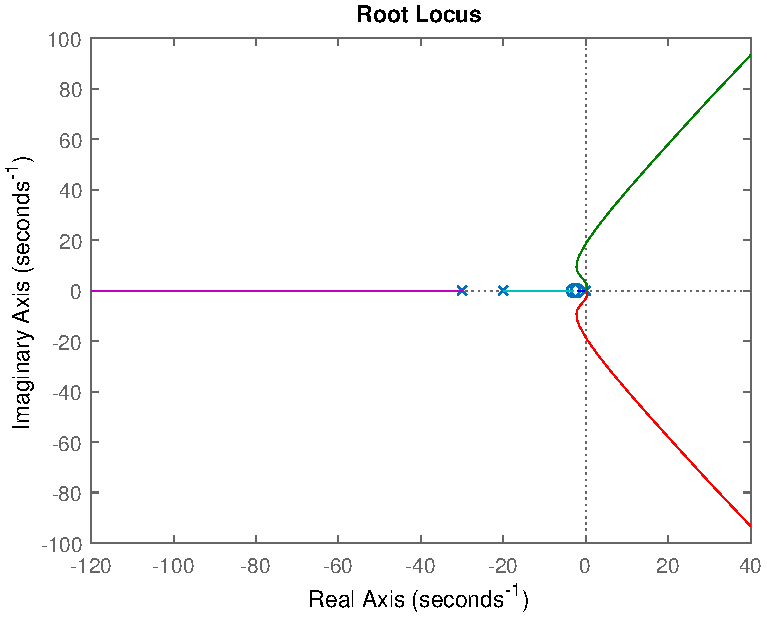
\includegraphics[width=3.5in]{problem3d.pdf}
    \end{center}
\end{figure}
The gain values associated with the \(j\omega\) axis crossings are approximately \(0.25\) and \(3.5\) which agrees
with my earlier results.

\paragraph{e)}

The bode plot is shown below.
\begin{figure}[H]
    \begin{center}
        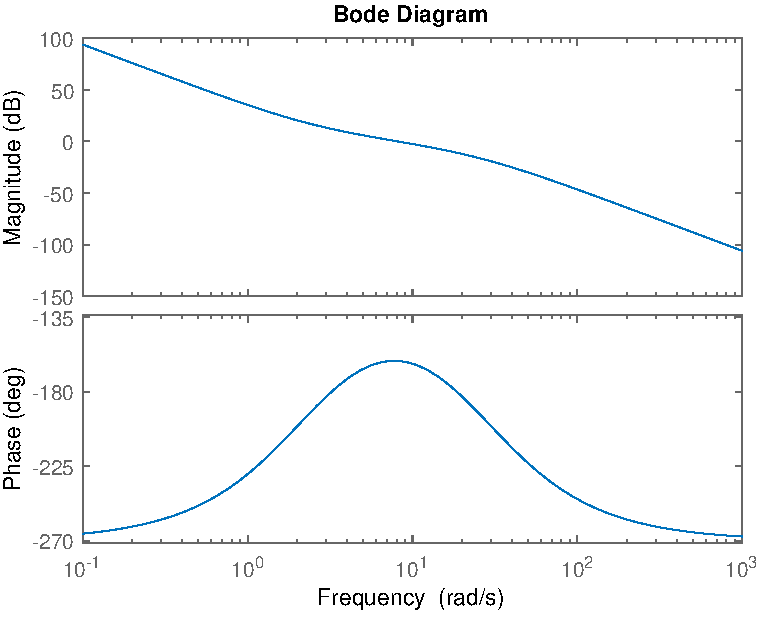
\includegraphics[width=3.5in]{problem3e.pdf}
    \end{center}
\end{figure}
At the crossover frequency of \(3.23\) radians per second, we have a gain margin of \(-12.2\) dB which corresponds
to the downward gain margin. At the crossover frequency of \(18.6\) radians per second, we have a gain margin of
\(10.9\) dB which corresponds to the upward gain margin. At the crossover frequency of \(8.17\) radians per
second we have a phase margin of \(18.6\) degrees.

\section*{Problem 4}

\paragraph{a)}

We want the intersection of the Nyquist diagram with the unit circle to be at \(-\frac{\sqrt{2}}{2}\pm j\frac{\sqrt{2}}{2}\)
in order for the phase margin to be 45 degrees. Then we can solve the following equation.
\begin{align*}
    \frac{K_p}{j\omega(j\omega+1)}&=-\frac{\sqrt{2}}{2}+ j\frac{\sqrt{2}}{2}\\
    \frac{K_p}{-\omega^2+j\omega}&=-\frac{\sqrt{2}}{2}+ j\frac{\sqrt{2}}{2}\\
    K_p&=\frac{\sqrt{2}}{2}(\omega^2-j\omega -j\omega^2 -\omega)\\
    K_p&=\frac{\sqrt{2}}{2}(\omega(\omega-1)-j\omega(\omega+1))\\
    K_p&=\sqrt{2}
\end{align*}
We set \(\omega=-1\) in order to make the imaginary term zero.

\paragraph{b)}

Since our phase margin is fairly low, we can use the approximate the damping ratio as \(\zeta=0.45\).
Then the approximate percent overshoot is given by the following equation.
\[e^{-\frac{\pi\zeta}{\sqrt{1-\zeta^2}}}=0.2053\]

\paragraph{c)}

The step response is shown below.
\begin{figure}[H]
    \begin{center}
        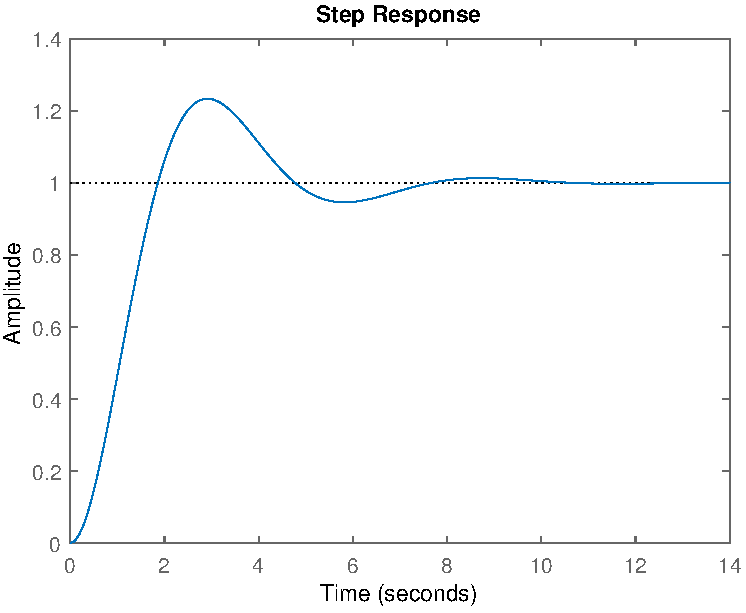
\includegraphics[width=3.5in]{problem4c.pdf}
    \end{center}
\end{figure}
The actual percent overshoot was \(0.233\) and the actual damping ratio is
\(\frac{1}{2^{1.25}}=0.42\). This is slightly lower than I predicted, leading to a slightly higher
percent overshoot.

\paragraph{d)}

The Nyquist diagram is shown below.
\begin{figure}[H]
    \begin{center}
        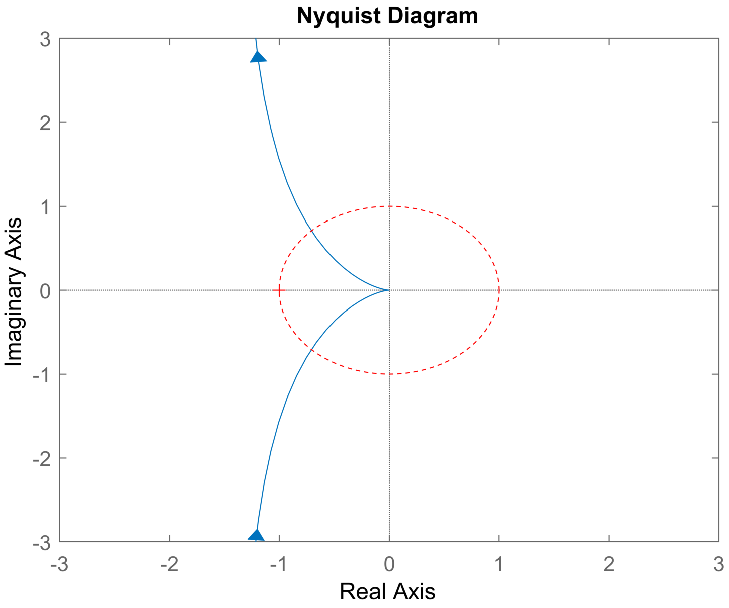
\includegraphics[width=3.5in]{problem4d.pdf}
    \end{center}
\end{figure}
This does indeed have a 45 degree phase margin since the Nyquist diagram lies on the line \(y=x\)
when it intersects the unit circle.

\section*{Problem 5}

\paragraph{a)}

My asymptote sketch and the actual bode plot is shown below.
\begin{figure}[H]
    \begin{center}
        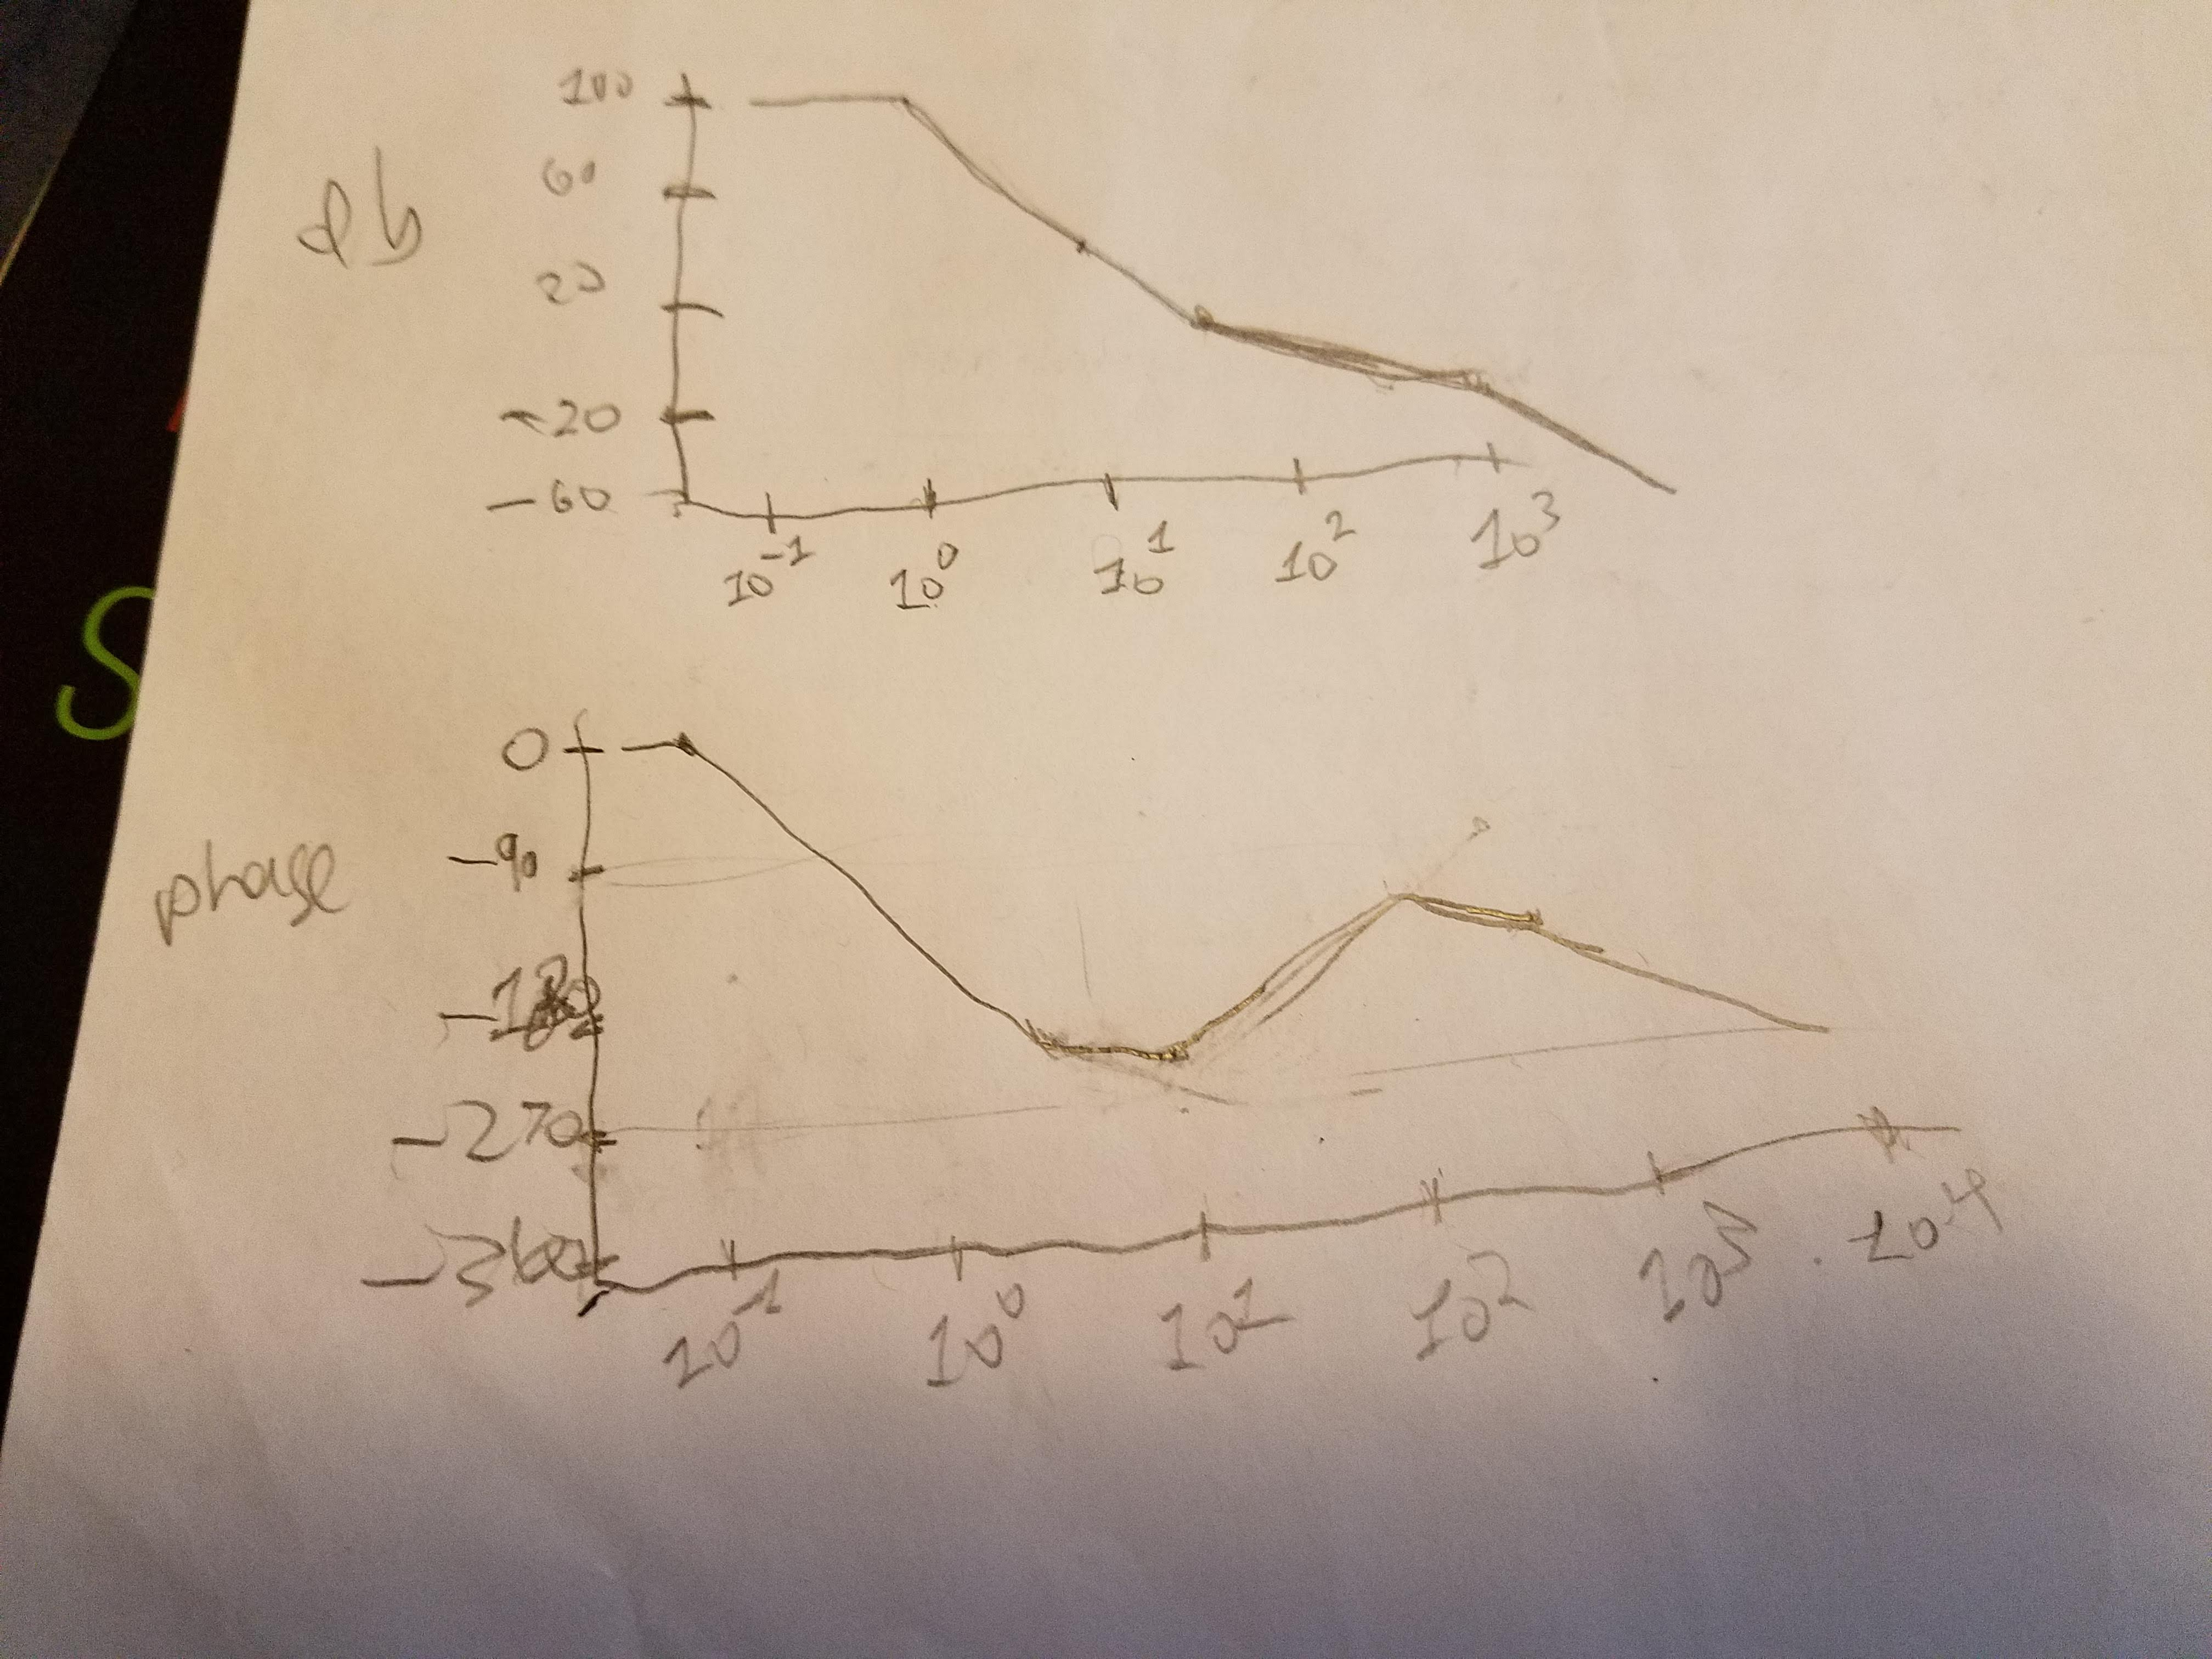
\includegraphics[width=2.5in]{problem5a.jpg}
        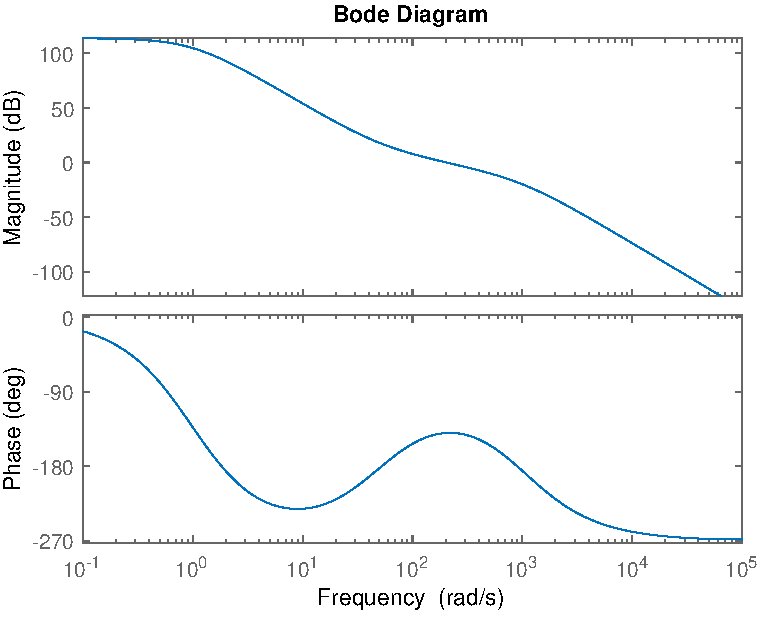
\includegraphics[width=2.5in]{problem5a.pdf}
    \end{center}
\end{figure}

\paragraph{b)}

The phase curve crosses \(-180\) degrees three times.

\paragraph{c)}

The bode plots are shown below.
\begin{figure}[H]
    \begin{center}
        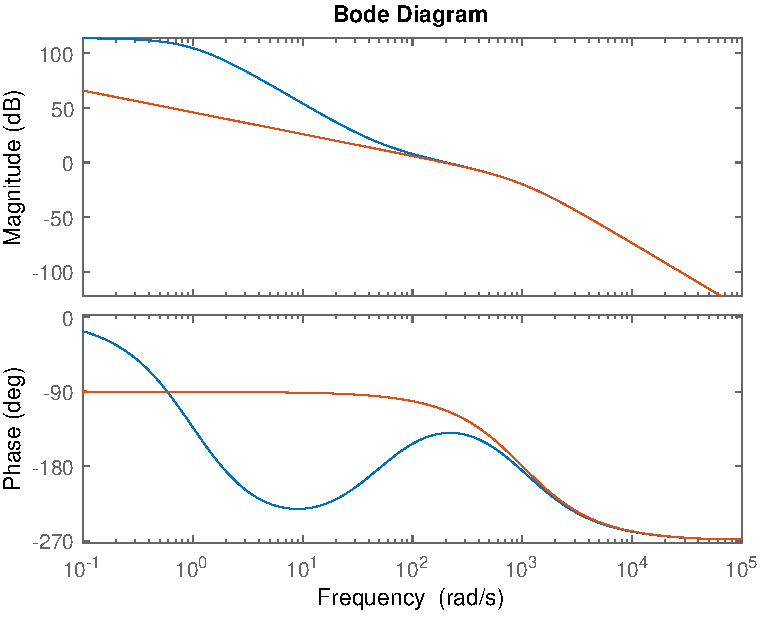
\includegraphics[width=3.5in]{problem5c.pdf}
    \end{center}
\end{figure}
The bode diagrams differ for lower frequencies because the first plot has a higher initial gain that decreases
faster as the frequency increases. The first transfer function also has more components than the simplified one,
so the phase moves up and down more. As the frequencies increase, both transfer functions perform similarly. The
first transfer function would have lower sensitivity at low frequencies in the closed loop system because its
gain is higher.

\paragraph{d)}

For \(L(s)\), the gain margin is -17.22 dB and the phase margin is 40.23 degrees. For \(L_2(s)\), the gain margin is
20 dB and the phase margin is 68.17 degrees. Here we can see that the larger gain and phase margins for \(L_2(s)\) allow
for better stability than \(L(s)\).

\paragraph{e)}

The upward gain margin of \(L(s)\) is 18.1 dB at a crossover frequency of 897 radians per second.

\paragraph{f)}

The Nyquist diagram is shown below.
\begin{figure}[H]
    \begin{center}
        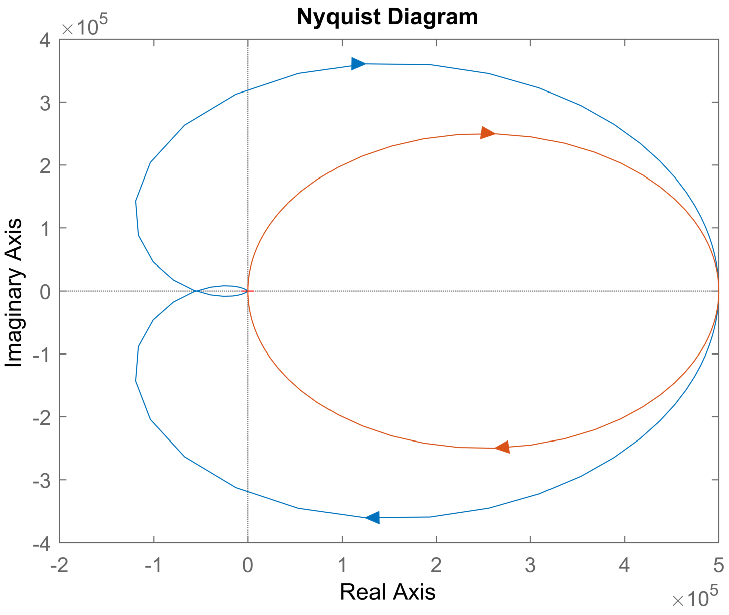
\includegraphics[width=3.5in]{problem5f-1.pdf}
    \end{center}
\end{figure}
Around the critical point, the Nyquist diagram looks like the following image.
\begin{figure}[H]
    \begin{center}
        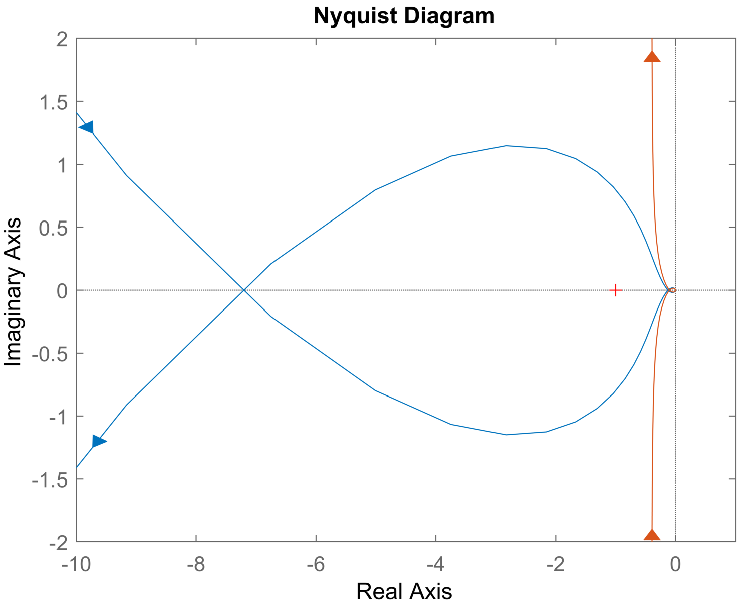
\includegraphics[width=3.5in]{problem5f-2.pdf}
    \end{center}
\end{figure}
The Nyquist diagram for \(L(s)\) does not encircle the critical point, since the inner loop is in the opposite direction
of the outer loop. The Nyquist diagram for \(L_2(s)\) does not encircle the critical point either, but it does not
cross the real axis at a point greater than the critical point. This means the downward gain margin is zero. It appears
to have a similar upward gain margin as \(L(s)\).

\end{document}